\section{Thermodynamik und Statistik: Erster Einstieg}
\subsection{Reversibilität und Irreversibilität}
Analytische Mechanik:
\begin{itemize}
    \item N Teilchen
    \item 3N Koordinaten $q_i(t), i=1, ..., 3N$
    \item 3N Impulse $p_i(t), i=1, ...., 3N$
 \end{itemize}

Phasenraumpunkt:
\begin{align}
    \vec{x} = \begin{pmatrix}q_1\\\vdots\\q_{3N}\\p_1\\\vdots\\p_{2N}\end{pmatrix}
    %Grafik von einem krummen Vektor
\end{align}
Hamiltongleichungen: 
\begin{align}
    \dot{q}_i &= \frac{\partial H}{\partial p_i} & \dot{p}_i &= - \frac{\partial H}{\partial q_i}
\end{align}


H: Hamiltonfunktion
Zeitumkehrinvariant $t \rightarrow -t$
Quantenmechanik:
\begin{align}
    i\hbar \partial_t \Psi(\vec{r}_1, \vec{r}_2, ..., \vec{r}_N, t) = \hat H (\Psi\vec{r}_1, ..., \vec{r}_N, t)
\end{align}

Zeitumkehrinvarianz:
\begin{align}
    \Aboxed{-i\hbar \partial_t \Psi^{*} = H \Psi^{*}}
\end{align}

\begin{figure}[H]
  \centering
  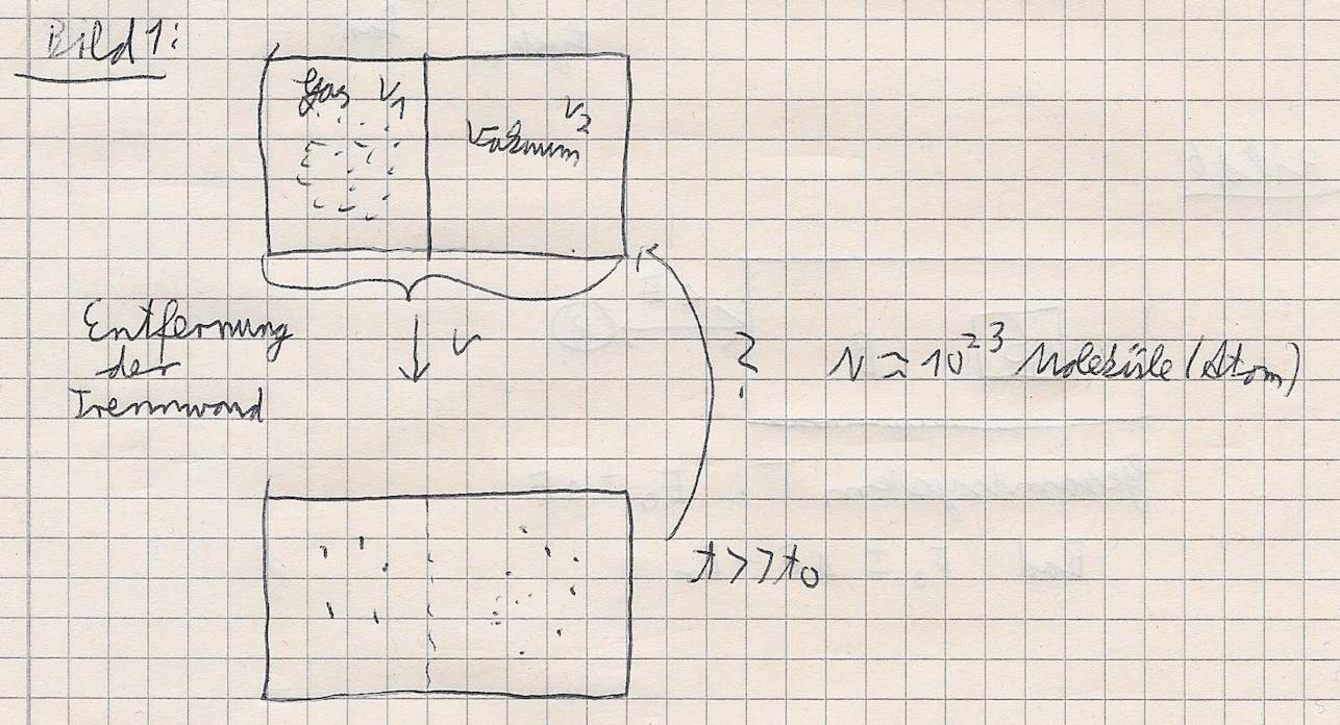
\includegraphics[width = \textwidth]{Zeichnungen/Bild1.pdf}
  \caption{Irreversibilität.}
  \label{fig:Bild1}
\end{figure}

\begin{itemize}
    \item Reversibel: Ein Prozess lässt sich spurlos umkehren.
    \item Irreversibel: Ein Prozess, der in der Umgebung eine Spur hinterlässt.
\end{itemize}
\enquote{Messfehler}: Auflösungsgrenze in Raum und Zeit.
$\Rightarrow$ Mittelungen

\begin{figure}[H]
  \centering
  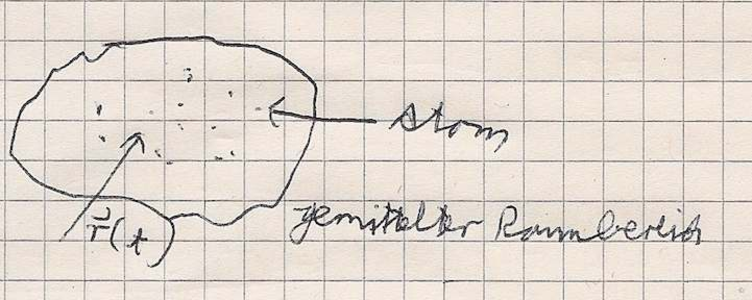
\includegraphics[width = \textwidth]{Zeichnungen/Bild2.pdf}
  \caption{Atome in Raumbereich.}
  \label{fig:Bild2}
\end{figure}
\subsection{ETH: Eigenzustand-Thermalisierungshypothese}

\begin{figure}[H]
  \centering
  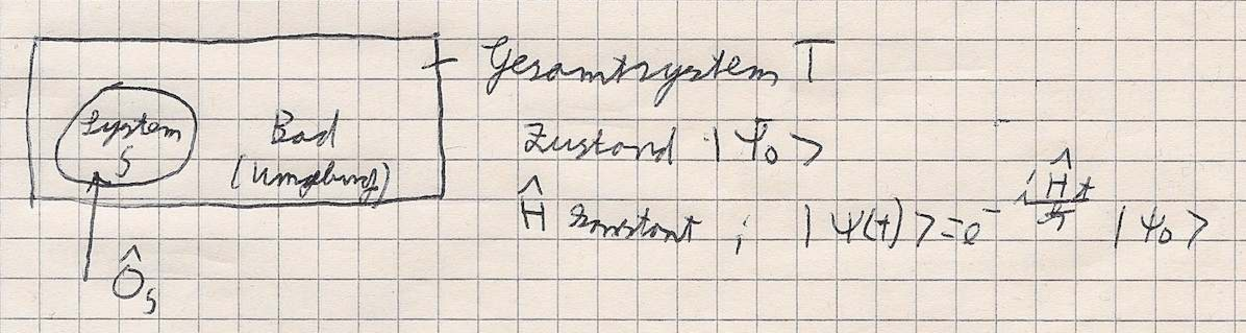
\includegraphics[width = \textwidth]{Zeichnungen/Bild3.pdf}
  \caption{Gesamtsystem und betrachtetes System.}
  \label{fig:Bild3}
\end{figure}

\begin{align}
    \Braket{O_S (t)} &= \Braket{\psi(t)|\hat{O_S} |\psi(t)}\\
    &= \Braket{\Psi_0| \symup{e}^{\frac{i H t}{\hbar}} O_S\,
    %\hat{1} = \sum_k |n><n|
    \symup{e}^{-\frac{i H t}{\hbar}}|\psi_0}\\
    &= \sum_k \Braket{\Psi_0 | \symup{e} ^ {-\frac{iHt}{\hbar}} | k} \Braket{k| \hat O_S \symup{e}^\frac{-iHt}{\hbar} | \Psi_0}\\
    &= \sum_k \langle k| \hat O_S \symup{e} ^ {-\frac{iHt}{\hbar}} \underbrace{| \Psi_0 \rangle \langle\Psi_0|}_{\hat \rho_0} \symup{e} ^ {-\frac{iHt}{\hbar}}|k\rangle\\ %\hat{rho}_0 &= |\Psi_0><\Psi_0|
    &= \sum_k \Braket{k| \hat O_S \symup{e} ^ {-\frac{iHt}{\hbar}} \rho_0 \symup{e} ^ {\frac{iHt}{\hbar}} | k}\\
    &= \Tr[\hat O_S \rho(t)]
\end{align}

\begin{align}
   \rho(t) &= \symup{e}^{-\frac{i H t}{\hbar}} \rho_0 \symup{e}^{\frac{i H t}{\hbar}}\\
    \hat \rho_0 \hat \rho_0 &= \hat \rho_0^2 = \hat \rho_0 \\
    \hat \rho_0^2 &\neq \hat \rho_0 \quad \text{Gemisch} 
\end{align}

Eigenbasis zu $\hat H$: \\
\begin{equation}
    \hat H \Ket{E_n} = E_n \Ket{E_n}
\end{equation}

\begin{align}
    \Braket{O_S(t)} &= \sum_{n,m} \Braket{E_n| O_S|E_m}
    \Braket{E_m| \symup{e}^{-\frac{i H t}{\hbar}} \rho_0 \symup{e}^{\frac{i H t}{\hbar}} |E_n}
\end{align}

\begin{align}
   \Aboxed{\Braket{O_S(t)} &= \sum_{k,m} = O^S_{n m} \rho_{m, n}^0 \symup{e}^{\frac{i}{\hbar} (E_n-E_m)t}}
\end{align}


System T: 
\begin{itemize}
    \item $N \sim10^{23} \rightarrow \infty$
    \item $E_N \rightarrow \infty$ (groß)
\end{itemize}

\begin{figure}[H]
  \centering
  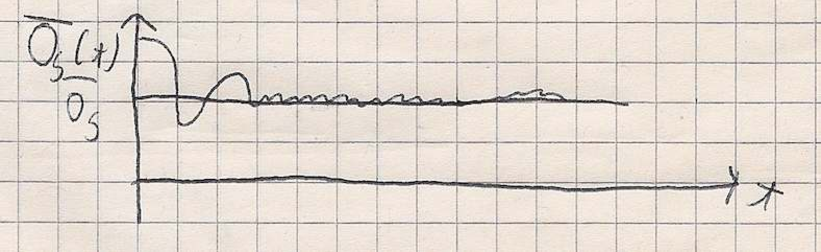
\includegraphics[width = \textwidth]{Zeichnungen/Bild4.pdf}
  \caption{Zeitlicher Verlauf von $O_S(t)$.}
  \label{fig:Bild4}
\end{figure}

\begin{align}
   \overline{O_S} &= \lim_{T \rightarrow \infty} \frac{1}{T} \int^T_0 \, \symup{d}t \Braket{O_S(t)} \\
    &= \sum_{n, m} O^2_{n, m} \rho^0_{mn} \underbrace{\lim\limits_{T \to \infty}\frac{1}{T} \int_0^T \symup{d}t
    \symup{e}^\frac{i(E_n - E_m) t}{\hbar}}_{\delta_{E_n, E_m}} \\
    \overline{O_S} &= \sum_{n,m} O^S_{n,m} \underbrace{\rho^0_{m,n} \delta_{E_n, E_m}}_{\bar\rho_{m,n}}\\
    &= ... = \Tr [\hat{O_S} \underbrace{\hat{\bar\rho}]}_\text{effektiver Dichteoperator}
\end{align}





$\Rightarrow$ Scharmittel\\
Zeitmittel $\hat{=}$ Scharmittel


\begin{align}
    \overline{\rho_{n,m}} &\equiv \rho^0_{n,m} \delta_{E_n, E_m} \Rightarrow [\hat{\bar\rho}, H] = 0 \\
    \bar{\rho}^2 &\neq \bar{\rho}\\
    [\bar\rho \vec\rho]_{n,m} &= \sum_k \bar \rho_{n, k} \bar \rho_{k,m} \\
    &= \sum_k \rho^0_{n,k} \rho^0_{k,m} \underbrace{\delta_{E_n, E_k} \delta_{E_k, E_m}}_{=\delta_{E_k, E_m}} \neq \bar \rho_{n, k}
\end{align}

$\Rightarrow$ Es entsteht ein Gemisch.

%Kasten drum
\begin{align}
    \bar{\rho} &= \sum_r \bar{\rho}\Ket r \Bra r%bis hier
    , \sum_r \bar{\rho_r} = 1
\end{align}

ETH: $\bar\rho$ Thermodynamischer Dichteoperator

\begin{figure}[H]
  \centering
  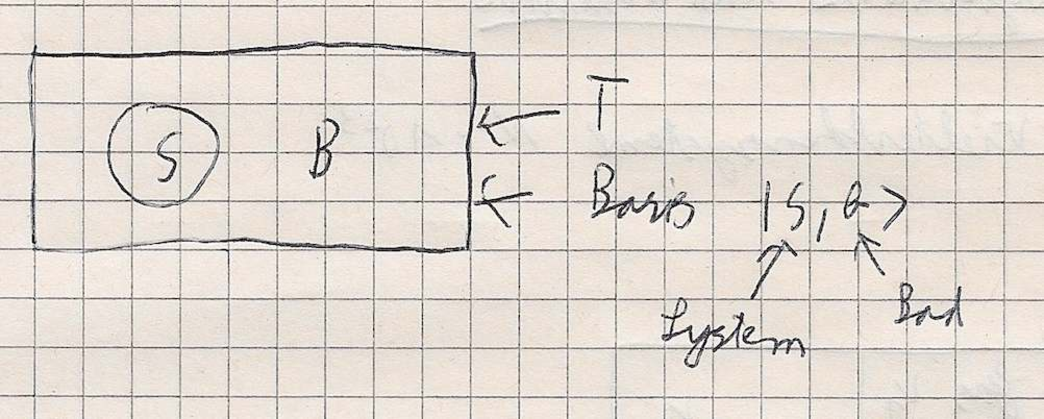
\includegraphics[width = \textwidth]{Zeichnungen/Bild5.pdf}
  \caption{System und Basis.}
  \label{fig:Bild5}
\end{figure}

\begin{align}
    \Ket{\Psi_0} &= \sum_{s,b} c_{s,b} \Ket{s,b} ,& \Braket{s,b|\hat O_S | s', b'} &= \delta_{b,b'} \Braket{s|\hat O_S|s'}\\
    \Braket{\Psi_0| \hat O_S |\Psi_0} &= \sum_{s, b}\sum{s', b'} c^{*}_{s,b} c_{s',b'} \Braket{s, b|\hat O_S| s', b'} \\
    &= \sum{s,s'} \Braket{s|\hat O_S|s'} \underbrace{\sum_b c_{s'b} c^{*}_{bs}}_{\rho^\text{red}_{s's}} \\
    &= \sum{s, s'} O^S_{s, s'} \rho^{\text{red}}_{s', s} \\
    [\rho^\text{red}]^2 &\neq [\rho^\text{red}]
\end{align}

\subsection{Gleichgewicht und Quantenstatistik}

\begin{align}
    \rho_{E_n} &= \rho_{E_m}, \quad \text{falls } E_n = E_m\\
    &= \rho(E)
\end{align}

\begin{figure}[H]
  \centering
  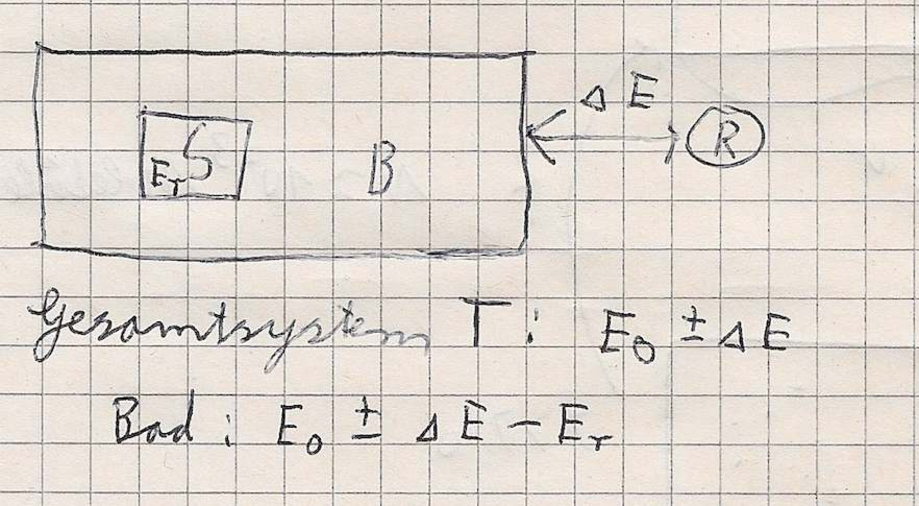
\includegraphics[width = \textwidth]{Zeichnungen/Bild6.pdf}
  \caption{System und Restsystem.}
  \label{fig:Bild6}
\end{figure}

\begin{align}
    \text{Gesamtsystem T: } E_0 &\pm \Delta E\\
    \text{Bad: } E_0 &\pm \Delta E - E_r = H_r\\
    \text{\#Zustände mit } H_r = E_0 &\pm \Delta E - E_r \eta (H_r) 2 \Delta E
\end{align}

\begin{align}
    \frac{\rho^S(E_r)}{\rho^S(E_{r'})} = \frac{\eta(H_r)}{\eta(H_{r'})} = \symup{e} \\
    E_0 \gg E_r, E_{r'} \\
    \frac{\symup{d}}{\symup{d}E} \ln \eta(E) = \beta(E_0) \stackrel{~}{~} \text{const.} \\
    \rho^S(E_r) = 1/Z \symup{e}^{-\beta E_r}, Z  = \sum_r \symup{e}^{-\beta E_r}
\end{align}

\subsection*{Wiederholung}
Zeitmittel $\hat{=}$Scharmittel
\begin{align}
    \overline{O_S} &= \lim\limits_{T \to \infty} \frac{1}{T} \int_0^T \symup{d}t \, \Braket{\underbrace{\hat O_S(t)}_{\Tr[\hat \rho_0 \hat O_S(t)]}} \\
    &= \Tr[\overline{\rho} \hat O_S(t)]\\
    &= \Tr[\hat O_S \overline \rho]
\end{align}

\begin{align}
    [\hat{\overline\rho}, \hat H = 0], \text{aber}\, [\hat O_S, \overline{\rho} \neq 0]
\end{align}


\begin{align}
    \hat \rho_0 &= \Ket{\Psi_0} \Bra{\Psi_0}
\end{align}

\begin{align}
    \overline{\rho} \neq \Ket{r}\Bra{r},\ \text{da}\ \overline{\rho}_{s,s'} \rightarrow  \text{Diagonalisierung} \rightarrow \rho_r : \overline{\rho} = \underbrace{\sum_{r} \rho_r \Ket{r}\Bra{r}}_{\text{Spektralzerlegung}} 
\end{align}

%Bild7

\begin{align}
    \Longrightarrow \Aboxed{\sum_{r}\rho_r=1}
\end{align}

%Bild8

\begin{align}
    \text{Gesamtsystem hat die Energie} &E_0\pm \increment E\\
    \text{System S:}\ &E_r\\
    \Rightarrow \text{Bad B:}\ &H_r=E_0-E_r\pm \increment E
\end{align}

Wahrscheinlichkeit für die Energie $E_r$: $\rho_s(E_r)$\\
\# Anzahl der Kombinationen (Zustände) mit Energie $H_r$ im Bad:

\begin{align}
    = \eta(E_0-E_r) 2 \increment E \\
    \increment E \to 0 \, \text{für} \, N \to \infty  
\end{align}



\begin{align}
    \frac{\rho_s(E_r)}{\rho_s(E_{r'}} 
    &= \frac{\eta(E_0-E_r)\cancel{2 \increment E}}{\eta(E_0-E_{r'})\cancel{2\increment E}} \\
    &= \symup{e}^{\ln \eta (E_0 - E_r) - \ln \eta (E_0 - E_{r'})}\\
    &\approx \symup{e}^{\beta (E) (-E_r + E_{r'})}\\
    &= \symup{e}^{-\beta  (E_r - E_{r'})}\\
    E_0 &\gg E_r, E_{r'} \\
\intertext{Nebenrechnung, Taylorreihe: }
    \ln \eta(E_0-E_r) &= \ln \eta(E_0) + 
    \underbrace{\frac{\symup{d}}{\symup{d}E} \ln\eta(E) \bigg|_{E_0}}_{\beta(E)} 
    (E_0 - E_r) + O((E_0 - E_r)^2) \\
    [\beta(E)] &= [\frac{1}{E}]
\end{align}

% Weiß jemand was das hier ist ?????????? nebenrechnung
\begin{align}
    \sum_{r} \rho(E_r) = 1 \\
    \rho(E_r) \propto \symup{e}^{-\beta(E) E_r}
\end{align}

\begin{align}
    \intertext{Zustandssumme Z}
    Z=\sum_{r}^{} e^{-\beta E r} = e^{-\beta F}\\
    \intertext{Parametrisierung der Zustandssummen mit F : Helmholtzsche \enquote{Freie Energie}}
    \Rightarrow \rho(E_r) = \frac{1}{Z} \symup{e}^{-\beta E_r}
\intertext{Mit der Annahme $\beta(E) \approx$ konst.}
    \beta &=\frac{1}{k_\text{B}T} \\
\end{align}

\begin{align}
    T:& \text{Temperatur}\\
    k_\text{B}:&\text{Boltzmankonstante} 
\end{align}

Freie Energie
\begin{align}
F = - \frac{1}{\beta} \ln (Z) = F(T,V)\\
T : \text{intensive Größe}\\
V: \text{extensive Größe} \Rightarrow V \propto N\\
F: \text{extensive Größe}
\end{align}
Additivität von Teilsysteme $A+B$   

\begin{align*}
%    \Aboxed{{\Aboxed A} {\Aboxed B}} % geht nichzt :(
\end{align*}

\begin{align}
    \rho{A+B} &= \frac{1}{Z_{A+B}}\symup{e}^{-\beta E}\\
    &= \rho_A(E_A)\ \rho_B(E_B) \\
    &= \frac{1}{Z_A Z_B} \symup{e}^{-\beta(E_A + E_B)}\\
\text{mit:}\, E = E_A + E_B
    \rightarrow Z_{A+B}&=Z_A Z_B\\
    \rightarrow F_{A+B}&=-\frac{1}{\beta}\ln(Z_{A+B})=F_A F_B :\text{F ist additiv}
\end{align}

\subsection{Einführung der Entropie}
Innere Energie $U$ 


\begin{align}
    U=\Braket{\hat H_S}% &= \Tr[\overline{\rho}\hat H_S]\\
    &=\sum_{r}\frac{\symup{e}^{-\beta E_r}}{Z} E_r \\
    &= -\frac{\partial}{\partial \beta} \ln Z\\
    U-F &=\frac{1}{Z} \sum_{r} e^{-\beta E_r} E_r \frac{\beta}{\beta} + \frac{1}{\beta} \ln Z 
    \left(\frac{1}{Z} \sum_{r} e^{-\beta E_r} \right) \\
    &= \frac{-1}{Z\beta} \sum_r e^{-\beta E_r} \underbrace{-\beta E_r -\ln Z}_{\underbrace{\ln(e^{-\beta E_r - \ln Z})}_{\rho(E_r)}}\\
    &=T(-k_\text{B}) \sum_{r} \rho(E_r) \ln \rho(E_r) = \text{TS}
\end{align}


mit der Entropie S
\begin{align*}
    S &= -k_\text{B} \sum_r \rho (E_r ) \ln \rho(E_r) \leq  0 \\
    1\leq \rho &\leq 0 \\
    \ln(x) &\geq 0 \ \text{Für}\ x\geq 1  \\
    \Aboxed{U&\leq F} \\
    \Rightarrow F(T,U) = U-TS \,\,\,\,&\hat{=}\,\,\,\, U =F+TS
\end{align*}

\subsection*{Wiederholung?}
\begin{align}
\intertext{Freie Energie}
    F(T, V) &= - \frac{1}{\beta} \ln Z, \frac{1}{\beta} = k_\text{B} T \\
\intertext{Zustandssumme}
    Z &= \Tr[\symup{e}^{-\beta \hat H}] = \sum_n \symup{e}^{-\beta E_n} = \symup{e}^{-\beta F} \\
\intertext{Innere Energie}
    U &= \Braket{\hat{H}}=\frac{1}{z} \sum_{n}e^{-\beta E_n} E_n \\
    U-F&=TS=T\left(-k_\text{B}\sum_{n} \underbrace{\frac{1}{z}e^{-\beta E_n}}_{\rho_n} \ln(\rho_n)\right)
\intertext{Entropie}
    S &= -k_\text{B} \sum_n \rho_n \ln \rho_n = - k_\text{B} \Braket{\ln\rho_n}\\
    S[\hat\rho] &= -k_\text{B} \Tr[\hat\rho \ln\hat\rho]
\intertext{Totales Differential}
    \symup{d} F &= \left(\frac{\partial F}{\partial V}\right)_T \symup{d} V +
    \left(\frac{\partial F}{\partial T}\right)_V \symup{d} T\\
    - \left(\frac{\partial F}{\partial T}\right)_V  &= \partial_T (U_B T \ln Z) = \frac{k_\text{B} T}{T} \ln Z + k_\text{B} T \frac{1}{Z} \frac{\partial}{\partial T} Z\\
    \frac{\partial}{\partial T} &= \frac{\partial \beta}{\partial T} = -k_\text{B} \beta^2 \frac{\partial}{\partial \beta}\\
    &= - \frac{1}{T} F + \frac{1}{T} \underbrace{\frac{1}{Z} \sum_n (+E_n) \symup{e}^{-\beta E_n}}_{U}\\
    -\left(\frac{\partial F}{\partial T}\right)_V&=\frac{1}{T}(U-F)=S \\
    (\frac{\partial F}{\partial V})_T &= -P\\
    \left[-\frac{\partial H}{\partial x}\right] &\propto [\text{Kraft}]\\
    \left[-\frac{\partial H}{\partial V} \right]&=\left[ \frac{\mathrm{Kraft}}{\mathrm{Fläche}}\right]=P\ (\mathrm{Druck}) 
\end{align}

\underline{Genauer:}
\begin{align}
    - \pdif{F}{V}[T] &= \frac{1}{\beta} \pdif{}{V} \ln Z=  \frac{1}{\cancel{\beta}} \frac{1}{Z} \sum_n \left(-\cancel{\beta} \frac{\partial}{\partial V} E_n\right) \symup{e}^{-\beta E_n} = -\frac{1}{Z} \sum_n \symup{e}^{-\beta E_n} \pdif{E_n}{V}[]\\
    &= - \Braket{\frac{\partial H}{\partial V}} \geq 0 \\
\intertext{Beispiel: Potentialtopf:}
    E_n &= \frac{\pi^2 \hbar^2}{2m} \frac{n^2}{L^2} \propto \frac{1}{V^{\sfrac{2}{a}}} \\
    \pdif{E_n}{V} &\propto - \frac{2}{a} \frac{1}{V} \frac{1}{V^{\sfrac{2}{a}}} 
\end{align}
\begin{align}
    \symup{d} F &= -p\symup{d} V- S \symup{d}T\\
    F &= U-TS\\
    U &= F +TS\\
    \symup{d}U &= \symup{d}F + \symup{d}(TS) = (-p \symup{d}V - S \symup{d} T) + T \symup{d}S + S \symup{T}\\
    &= -p \symup{d}V + T \symup{d}S\\
    \Rightarrow U &= U(V,S)  \quad \text{U ist Legendre-Transformatierte von}\ F(V,T)
\end{align}
\begin{align}
    \Aboxed{\left(\frac{\partial U}{\partial S} \right)_V = T} \geq 0 \quad \text{d.h. Definition der Temperatur}
\end{align}

\subsection{Interpretation des Entropie-Begriffs}

\begin{align}
    S &= - k_\text{B} \sum_n \rho_n \ln \rho_n = -k_\text{B} \Tr[\hat \rho \ln\hat\rho]
\end{align}
Beispiel: Spin-System mit M Spin 1/2 : Hilbertraum -Dim.: $D=2^M$
\begin{align}
    M = 4 \Rightarrow D = 2^4 = 16
\end{align}
Anzahl der Fragen zum Zustandsrest:

%Bild 9

Informationsinhalt: $ M = \log_2 D$
\begin{align}
    \# \text{Fragen} &\propto \ln D\\
    \text{Gleichverteilung:  }\rho_n &= \frac{1}{D}\\
    S &= -k_\text{B} \underbrace{\sum_n \rho_n}_{=1} \cdot \ln \frac{1}{\beta} = k_\text{B} \ln D\\
\end{align}
Entropie: Maß für unser Unwissen über das System
Wir maximieren die Entropie
\begin{align}
    S[\hat \rho] &= -k_\text{B} \Tr [\hat \rho \ln \rho]\quad \text{Funktional}\\ 
\intertext{Nebenbedingung}
    \Tr[\hat \rho] &= 1 = \sum_n \rho_n \\
    I[{\rho_n}] &= S [{\rho_n}] + k_\text{B} \lambda_0 \left(\sum_n \rho_n -1\right)\\
    \delta I &= 0\\
    \Rightarrow \frac{I}{\rho_n} &= - k_\text{B} \frac{\partial}{\partial \rho_n} \left[\sum_n \rho_{n'} \ln \rho_{n'} - \lambda_0\left(\sum_n \rho_n -1\right)\right]\\
    &=  -k_\text{B} [ \underbrace{\ln \rho_n +1}_{= 0} - \lambda_0] = 0 \\
    \Rightarrow \rho_n &= \symup{e}^{\lambda_0 -1} \quad \text{Gleichverteilung}
\end{align}
\begin{align}
    \sum_n \rho_n = 1 = \sum^D_{n=1} \symup{e}^{\lambda_-1} &= \symup{e}^{\lambda_-1}D \Rightarrow \symup{e}^{\lambda_-1} = \frac{1}{D} = \rho_n\\
    \intertext{Maximum ?}
    \eta(x) &= -x \ln x \\
    \eta' (x) &= -(\ln x +1)\\
    \eta''(x) &= - \frac{1}{x} \quad < 0 \quad x > 0\quad \text{Maximum}
\end{align}

\subsection{von-Neumann-Gleichung}

\begin{align}
    i \hbar \partial_t \Ket{\Psi} &= \hat H \Ket{\Psi}\\
    \hat \rho (t) &= \sum_n p_n \Ket{n(t)} \Bra{n(t)}\\
    i \hbar \Ket{n(t)} &= \hat H \Ket{n(t)}\\
    - i \hbar \Bra{n(t)} &= \Bra{n(t)} H\\
    \frac{\partial}{\partial t}\hat\rho(t) &= \sum_n P_n \left[\left( \frac{\partial}{\partial t} \Ket{n(t)}\right) \Bra{n(t)} + \Ket{n(t)} \left( \frac{\partial}{\partial t} \Bra{n(t)} \right) \right]\\
    &= \frac{1}{i \hbar} \sum_n p_n \left[\hat H \Ket{n(t)} \Bra{n(t)} - \Ket{n(t)} \Bra{n(t)} \hat H\right] \\
    \Aboxed{
        \frac{\partial \rho (t)}{\partial t} &= \frac{i}{\hbar} \left[\hat \rho(t), \hat H \right]
    }  \quad \text{von-Neumann-Gleichung}
\end{align}


\subsection{Wahrscheinlichkeitsverteilung und zentraler Grenzwertsatz}

Würfel: Mit welcher Wahrscheinlichkeit würfel' ich die Zahl $X$ \\
Antwort: $P$


\begin{align}
    N &\ \text{Ereignisse} \\
    Q: w_N(n) &= p^n (\underbrace{1-p}_{q})^{N-n}
\intertext{$n$ mal die Zahl $X$ zu finden:}
    \sum_{n=0}^{N} w(n) &= \sum_{n=0}^N \binom{N}{n} p^n q^{N-n} = (\underbrace{p+q}_{=1})^N = 1\\
    N\to\infty
\end{align}
\subsubsection*{Statistische Verteilungsfunktion für eine kontinuierliche Variable $X: w(x)$}
Statistische Mittelung von $f(x)$
\begin{align}
    \Braket{f} &= \int_{-\infty}^\infty \symup{d}x w(x)f(x) \quad \left[ \Braket{f} = \frac{1}{N} \sum^N_{i=1} f(x_i) \right]\\
    p(x) &= w(x)\symup{d} x, \quad x\in[x,x+\symup{d}x] \\
    \intertext{Normierung}
    \Braket{1}&= \int_{-\infty}^\infty \symup{d}x w(x)=1
\end{align}
\paragraph{Charakteristische Funktion:}
\begin{align}
    \tilde w(k) &= \Braket{\symup{e}^{-ikx}} = \int_{-\infty}^\infty \symup{d} x w(x) \symup{e}^{-ikx} \quad \text{FT von}\ w(x) \\
    \Rightarrow w(x)&=\int_{-\infty}^\infty \frac{\symup{d}k}{2\pi}\ \tilde w(x) e^{ikx} \\
    \Rightarrow \tilde w(0)&=1 \quad \text{(Normierung)}
\end{align}

\paragraph{Taylor-Reihe}
\begin{align}
    \tilde w(k) &= \Braket{\sum^\infty_{n=0} \frac{(-ik)^n}{n!} x^n}
    =\sum_{n=0}^{\infty} \frac{(-ik)^{n}}{n!} \underbrace{\Braket{x^n}}_{\text{Momente der Verteilung}}
\end{align}
Charakteristische Funktion enthält \emph{alle} Momente der Verteilung 
\begin{align}
    \Rightarrow \Braket{x^n} &= i^n \frac{\symup{d}^n}{\symup{d}k^n}\tilde w(k) \Bigg|_{k=0}
\end{align}
\paragraph{Kumulanten:}
Maß für Fluktuationen
\begin{align}
    \ln \tilde w(k)&=\ln \Braket{\symup{e}^{-i kx}} = \sum_{n=1}^\infty \frac{(-i k)^n}{n!} \Braket{x^n}_C\\
    \stackrel{\text{Taylorreihe}}{\Rightarrow} \Braket{x^n}_C &= i^n \frac{\symup{d}^n}{\symup{d}k^n}[\ln(\tilde w(k)] \bigg|_{k=0}\\
\end{align}
\begin{align}
    n=1&: \quad \Braket{x}_C = i\frac{\symup{d}}{\symup{d}k}[\ln \tilde w(k)]=i\frac{\tilde w'(k)}{\tilde w(k)}\bigg|_{k=0} = i \tilde w'(0) = \Braket{x} \\
    n=2&: \quad \Braket{x^2}_C = i^2 \frac{\symup{d}}{\symup{d}k} \left[\frac{\tilde w'(k)}{\tilde w(k)}\right]_{k=0} \\
    &\quad= i^2 \left[\frac{\tilde w''(k)}{\tilde w(k)}-\frac{\tilde w'(k)^2}{\tilde w(k)^2}\right]_{k=0}\\
    &\quad = [i^2 \tilde w''(k) - (i w')^2]_{k=0}\\
    \Aboxed{\Braket{x^2}_C &= \Braket{x^2}  \Braket{x}^2 = \sigma ^2} \quad \text{Kumulante 2. Ordnung}
\end{align}
\begin{align}
\intertext{Annahme:}
    \ln \tilde w (k) &\approx -i k\Braket{x} + \frac{(ik)^2}{2}\Braket{x^2}_C+O(\Braket{x^3}) \\
    \Rightarrow \tilde w(n) &= \symup{e}^{ik \Braket{x}+ \frac{(-ik)^2}{2}\Braket{x^2}_C}
\intertext{F.T.}
    w(x) &= \int_{-\infty}^\infty \frac{\symup{d}k}{2\pi} \symup{e}^{ikx} \symup{e}^{-ik \Braket{x} - \frac{k^2}{2} \Braket{x^2}_C}\\
    &= \int_{-\infty}^\infty \frac{\symup{d}k}{2\pi} \exp\left({-\frac{\Braket{x^2}_C}{2} \left[\underbrace{k^2-2i k \frac{x-\Braket{x}}{\Braket{x^2}_C} + \frac{[i (x -\Braket{x})]^2}{\Braket{x^2}_C^2}}_{\overline k ^2} - \frac{[i (x -\Braket{x})]^2}{\Braket{x^2}_C^2}\right]}\right)\\
    &= \exp\left({-\frac{1}{2}\frac{(x-\Braket{x})^2}{\Braket{x^2}_C}} \cdot \frac{1}{\sqrt{2 \pi \Braket{x^2}_C}}\right)\\
    \Rightarrow \text{Gaußverteilung}
\end{align}

%Bild 10

Charakteristische Funktion als diskrete Fourier-Transformation von $w_N(n)$
\begin{align}
    \tilde w _N (k) &= \Braket{\symup{e}^{-i kx}} = \sum_{n=0}^N w_N(k) \symup{e}^{-ikn}\\
    &= \sum_{n=0}^N \binom{N}{n} \underbrace{p^n q^{N-n}}_{(p\symup{e}^{-ik})^n} \symup{e}^{-ikn} = (p \symup{e}^{-ikn} +1)^N\\
    \Rightarrow \ln \tilde w(n) &= N \ln(p \symup{e}^{-ikn} +q)\\
\intertext{ $\Rightarrow$ alle Kummulanten $\propto N$ }
    \Braket{k} &= i\frac{d}{d k} \ln \tilde w'^(k)_N \bigg|_{k=0} = iN \frac{-ip \symup{e}^{-ik}}{p \symup{e}^{-ik}+q} \bigg|_{k=0} = N \cdot P\\
    \Braket{k^2}_C &= i \frac{\symup{d}}{\symup{d}k} \left[i N \frac{-i p \symup{e}^{-ik}}{p\symup{e}^{-ik +q}}\right] = ... = N p q = \sigma^2
\intertext{relative Abweichung}
\frac{\sigma}{\Braket{n}}&=\frac{\sqrt{\Braket{n^2}_c}}{\Braket{n}} =\frac{\sqrt{N p q}}{Np}=\frac{1}{\sqrt{N}}\sqrt{\frac{q}{p}}\propto \frac{1}{\sqrt{N}}\\
\intertext{Zentraler Grenzwertsatz:}
\intertext{intensive Größen:}
    x &= \frac{n}{N} \quad 0 \leq x \leq 1\\
    \bar x &= \frac{\Braket{n}}{N}=p ; \: \: \bar \sigma^2 = \frac{\sigma^2}{N}= pq\\
    w_N (n=N x) &= \frac{1}{\sqrt{2 \pi N \bar \sigma^2}} \symup{e}^{-\frac{1}{2}\frac{(x-\Braket{x^2})^2}{2 \frac{\overline \sigma^2}{N}}}\\
    w_N(n) \underbrace{\symup{d}n}_{N \symup d x} &= w_N(x) \symup{d}x \\
    \sigma_\text{eff.} &= \frac{\bar \sigma^2}{N} \rightarrow 0\\
    w_N(x) &= \frac{1}{\sqrt{2 \pi \frac{\overline{\sigma}^2}{N}}} \exp \left({-\frac{(x-\Braket{x})^2}{2 \overline \sigma^2/N}}\right)
\end{align}
\paragraph{Gesetz der großen Zahlen}
\begin{align}
    X&: X_1, X_2, ..., X_N \quad \text{Sequenz von Zufallszahlen}\\
    \mu &= E(X), \: \: \sigma^2 = \text{Var}(X)\\
    \intertext{Realisierung:}
    M &= \frac{1}{n} \sum^n_{k=1} X_n\\
    E[M]&=\mu \\
    \Var(M) &= \frac{\sigma^2}{n} \xrightarrow{n\to\infty} 0
\end{align}
\paragraph{Zentraler Grenzwertsatz}
\ \\
$X_1, X_2,...., X_n$ Reelle Zufallsvarianz der Gleichverteilung $w(X)$
\begin{align}
    Y_n &= \sum_{i=1}^{n} X_i\\
    \intertext{Mittelung}
    M_n &= \frac{Y}{n} \xrightarrow{n\to\infty} M \Rightarrow \Braket{Y_n} = nM = E[Y_n]\\
        &\Braket{Y_n^2}-\Braket{Y_n}^2=n\sigma^2\\
    \intertext{Normierung}
    Z_n &= \frac{Y_n-n\mu}{\sqrt{n}\sigma} \Rightarrow \Var(Z_n) = 1 \rightarrow w(Z) = \frac{1}{\sqrt{2\pi}} \symup{e}^{-\frac{1}{2}Z^2}
\end{align}